\begin{topic}{deutsch-jozsa-algorithm}{Deutsch--Jozsa algorithm}
    The \emph{Deutsch--Jozsa algorithm} is a quantum algorithm to solve the following problem:
    
    \textbf{Problem}: Given $x \in \{ 0, 1 \}^N$ for some $N = 2^n$, such that either all $x_i$ are equal (in this case, $x$ is called `constant'), or $N / 2$ of the $x_i$ are $0$ and $N / 2$ are $1$ (in this case, $x$ is called `balanced'). Determine whether $x$ is constant or balanced.
    
    \textbf{Algorithm}: Denote by $\mathcal{O}$ the query which acts as $\mathcal{O} \ket{i} = (-1)^{x_i} \ket{i}$ for all $i \in \{ 0, 1 \}^n$.
    \begin{enumerate}[label=(\arabic*)]
        \item Start with the $n$-qubit state $\ket{0^n}$.
        \item Apply a \tref{hadamard-gate}{Hadamard gate} to each qubit to obtain the state
        \[ \frac{1}{\sqrt{2^n}} \sum_{i \in \{ 0, 1 \}^n } \ket{i} . \]
        \item Apply the query $\mathcal{O}$ to obtain the state
        \[ \frac{1}{\sqrt{2^n}} \sum_{i \in \{ 0, 1 \}^n} (-1)^{x_i} \ket{i} . \]
        \item Apply a Hadamard gate to each qubit to obtain the state
        \[ \frac{1}{2^n} \sum_{i \in \{ 0, 1 \}^n} (-1)^{x_i} \sum_{j \in \{ 0, 1 \}^n} (-1)^{i \cdot j} \ket{j} . \]
        In particular, the amplitude of the $\ket{0^n}$-state in the final superposition is
        \[ \frac{1}{2^n} \sum_{i \in \{ 0, 1 \}^n} (-1)^{x_i} = \begin{cases}
            1 & \textup{if } x_i = 0 \textup{ for all } i , \\
            -1 & \textup{if } x_i = 1 \textup{ for all } i , \\
            0 & \textup{if } x \textup{ is balanced} .
        \end{cases} \]
        Measuring will yield $\ket{0^n}$ if $x$ is constant, and any other state if $x$ is balanced.
    \end{enumerate}
\end{topic}

\begin{topic}{bernstein-vazirani-algorithm}{Bernstein--Vazirani algorithm}
    The \emph{Bernstein--Vazirani algorithm} is a quantum algorithm to solve the following problem:
    
    \textbf{Problem}: Given $x \in \{ 0, 1 \}^N$ for some $N = 2^n$, such that $x_i = (i \cdot s) \mod 2$ for some unknown $s \in \{ 0, 1 \}^n$. The problem is to determine $s$.

    \textbf{Algorithm}: Denote by $\mathcal{O}$ the query which acts as $\mathcal{O} \ket{i} = (-1)^{x_i} \ket{i}$ for all $i \in \{ 0, 1 \}^n$.
    \begin{enumerate}[label=(\arabic*)]
        \item Start with the $n$-qubit state $\ket{0^n}$.
        \item Apply a \tref{hadamard-gate}{Hadamard gate} to each qubit to obtain the state
        \[ \frac{1}{\sqrt{2^n}} \sum_{i \in \{ 0, 1 \}^n } \ket{i} . \]
        \item Apply the query $\mathcal{O}$ to obtain the state
        \[ \frac{1}{\sqrt{2^n}} \sum_{i \in \{ 0, 1 \}^n} (-1)^{x_i} \ket{i} = \frac{1}{\sqrt{2^n}} \sum_{i \in \{ 0, 1 \}^n} (-1)^{i \cdot s} \ket{i} . \]
        \item Apply a Hadamard gate to each qubit to obtain the state $\ket{s}$.
        \item Measure the qubits to find $s$.
    \end{enumerate}
\end{topic}

\begin{topic}{simon-algorithm}{Simon's algorithm}
    \emph{Simon's algorithm} is a quantum algorithm to solve the following problem:

    \textbf{Problem}: Given $x = (x_0, \ldots, x_{N - 1})$ for some $N = 2^n$, where $x_i \in \{ 0, 1 \}^n$, with the property that there is some unknown non-zero $s \in \{ 0, 1 \}^n$ such that $x_i = x_j$ if and only if ($i = j$ or $i = j \oplus s$). Determine $s$.

    Note that $x$, viewed as a function from $\{ 0, \ldots, N - 1 \}$ to $\{ 0, \ldots, N - 1 \}$ is a $2$-to-$1$ function, whose $2$-to-$1$-ness is encoded by the unknown \textit{mask} $s$.

    \textbf{Algorithm}: Denote by $\mathcal{O}$ the query which acts as $\mathcal{O} \ket{i} \ket{y} = \ket{i} \ket{y \oplus x_i}$ for all $i \in \{ 0, 1 \}^n$.
    \begin{enumerate}[label=(\arabic*)]
        \item Start with the $2n$-qubit state $\ket{0^n} \otimes \ket{0^n}$.
        \item Apply \tref{hadamard-gate}{Hadamard gates} to the first $n$ qubits to obtain the state
        \[ \frac{1}{\sqrt{2^n}} \sum_{i \in \{ 0, 1 \}^n} \ket{i} \otimes \ket{0^n} . \]
        \item Apply the query $\mathcal{O}$ to obtain the state
        \[ \frac{1}{\sqrt{2^n}} \sum_{i \in \{ 0, 1 \}^n} \ket{i} \otimes \ket{x_i} . \]
        \item Measure the last $n$ qubits to obtain some value $x_i$. The state will now have collapsed to
        \[ \frac{1}{\sqrt{2}} (\ket{i} + \ket{i \oplus s}) \otimes \ket{x_i} . \]
        \item Apply Hadamard gates to the first $n$ qubits to obtain the state
        \[ \begin{aligned}
            \frac{1}{\sqrt{2^{n + 1}}} \left( \sum_{j \in \{ 0, 1 \}^n} (-1)^{i \cdot j} \ket{j} + \sum_{j \in \{ 0, 1 \}^n} (-1)^{(i \oplus s) \cdot j} \ket{j} \right) \\
            = \frac{1}{\sqrt{2^{n + 1}}} \left( \sum_{j \in \{ 0, 1 \}^n} (-1)^{i \cdot j} (1 + (-1)^{s \cdot j}) \ket{j} \right) .
        \end{aligned} \]
        \item Measure the first $n$ qubits to obtain some value $j \in \{ 0, 1 \}^n$. Since $\ket{j}$ has non-zero amplitude if and only if $s \cdot j \equiv 0 \mod 2$, this measurement yields a random element uniformly distributed from the set $\{ j \in \{ 0, 1 \}^n \mid s \cdot j \equiv 0 \mod 2 \}$. Such an element corresponds to a linear equation that gives information about $s$.
        \item Repeat the above until $n - 1$ linearly independent equations are obtained.
        \item Solve for $s$.
    \end{enumerate}
    Simon's algorithm uses $O(n)$ calls to $\mathcal{O}$, and polynomially in $n$ many operations to solve for $s$.
\end{topic}

\begin{topic}{kitaev-phase-estimation-algorithm}{Kitaev's phase estimation algorithm}
    Given a unitary $U$ and eigenvector $\ket{\psi}$ whose eigenvalue is $\lambda = \exp(2 \pi i \phi)$ for some $\phi \in [0, 1)$, \emph{Kitaev's phase estimation algorithm} is a quantum algorithm to compute $\phi$, given $U$ and $\ket{\psi}$.

    \textbf{Algorithm}: For simplicity, assume that $\phi$ can be expressed with $n$ bits of precision, that is, $\phi = \phi_1 / 2 + \phi_2 / 4 + \ldots + \phi_i / 2^n$.
    \begin{enumerate}[label=(\arabic*)]
        \item Start with the $2n$-qubit state $\ket{0^n} \otimes \ket{\psi}$.
        \item For $N = 2^n$, apply the \tref{quantum-fourier-transform}{quantum Fourier transform} $F_N$ to the first $n$ qubits to obtain the state
        \[ \frac{1}{\sqrt{N}} \sum_{j = 0}^{N - 1} \ket{j} \otimes \ket{\psi} . \]
        (Alternatively, applying the $n$-fold \tref{hadamard-gate}{Hadamard gate} $H^{\otimes n}$ has the same effect.)
        \item Apply the operation $\ket{j} \otimes \ket{\psi} \mapsto \ket{j} \otimes U^j \ket{\psi} = \exp(2 \pi i \phi j) \ket{j} \otimes \ket{\psi}$. This can be implemented, for instance, using controlled $U$ gates. This yields the state
        \[ \frac{1}{\sqrt{N}} \sum_{j = 0}^{N - 1} \exp(2 \pi i \phi j) \ket{j} \otimes \ket{\psi} . \]
        \item Apply the inverse quantum Fourier transform $F_N^{-1}$ to the first $n$ qubits to obtain the state
        \[ \ket{\phi_1 \phi_2 \cdots \phi_n} \otimes \ket{\psi} . \]
    \end{enumerate}
    The value of $\phi$ can now be obtained by measuring the first $n$ qubits.
\end{topic}

% \begin{topic}{shor-algorithm}{Shor's algorithm}
    
% \end{topic}

\begin{topic}{grover-search-algorithm}{Grover's search algorithm}
    \emph{Grover's search algorithm} is a quantum algorithm to solve the following problem:

    \textbf{Problem}: Given $x \in \{ 0, 1 \}^N$ for some $N = 2^n$, find some $i \in \{ 0, 1 \}^n$ such that $x_i = 1$.

    \textbf{Algorithm}: Denote by $\mathcal{O}$ the query which acts as $\mathcal{O} \ket{i} = (-1)^{x_i} \ket{i}$ for all $i \in \{ 0, 1 \}^n$. Denote by $R$ the unitary operation given by $R \ket{0^n} = \ket{0^n}$ and $R \ket{i} = - \ket{i}$ for $i \ne 0^n$. Define the \textit{Grover iterate} to be the operation $\mathcal{G} = H^{\otimes n} R H^{\otimes n} \mathcal{O}$, where $H$ is the \tref{hadamard-gate}{Hadamard gate}.
    \begin{enumerate}[label=(\arabic*)]
        \item Start with the $n$-qubit state $\ket{0^n}$.
        \item Apply a Hadamard gate to each qubit to obtain the uniform state
        \[ \ket{U} = \frac{1}{\sqrt{2^n}} \sum_{i \in \{ 0, 1 \}^n } \ket{i} . \]
        \item Write $\ket{U} = \sin(\theta_0) \ket{G} + \cos(\theta_0) \ket{B}$ for $\theta_0 = \arcsin(\sqrt{t / N})$ and
        \[ \ket{G} = \frac{1}{\sqrt{t}} \sum_{i \mid x_i = 1} \ket{i}, \quad \ket{B} = \frac{1}{\sqrt{N - t}} \sum_{i \mid x_i = 0} \ket{i} , \]
        where $t$ is the number of $x_i$ equal to $1$.
        \item Observe that the Grover iterate $\mathcal{G}$ is the composite of $\mathcal{O}$ and $H^{\otimes n} R H^{\otimes n} = 2 \ket{U} \bra{U} - I$. In the $2$-dimensional plane spanned by $\ket{G}$ and $\ket{B}$, this corresponds to a reflection through $\ket{B}$ followed by a reflection through $\ket{U}$. Therefore,
        \[ \mathcal{G}^k \ket{U} = \sin(\theta_k) \ket{G} + \cos(\theta_k) \ket{B} \quad \textup{ with } \theta_k = (2k + 1) \theta_0 \]
        for any $k \ge 0$.
        \item Choose $k$ such that applying $k$ Grover iterates maximizes the probability to measure some $i$ with $x_i = 1$. Explicitly, this probability is $P_k = \sin((2k + 1) \theta_0)^2$, so choose $k$ to be the integer closest to $\tilde{k} = \tfrac{\pi}{4} \theta_0 - \tfrac{1}{2}$.
        \item Apply $k$ Grover iterates and measure the qubits to obtain some $i$. The failure probability is
        \[ \begin{aligned}
            1 - P_k
                &= \cos((2k + 1) \theta_0)^2 = \cos((2 \tilde{k} + 1) \theta_0 + 2 (k - \tilde{k}) \theta_0)^2 \\
                &= \cos(\pi/2 + 2 (k - \tilde{k}) \theta_0)^2 = \sin(2(k - \tilde{k}) \theta_0)^2 \le \sin(\theta_0)^2 = \frac{t}{N} .
        \end{aligned} \]
    \end{enumerate}
    Since $\arcsin(\theta_0) \ge \theta_0$, the number of Grover iterates is $k \le \tfrac{\pi}{4} \theta_0 \le \tfrac{\pi}{4} \sqrt{N/t}$. When $t$ is unknown, the above algorithm is run for different guesses of $k$. The expected number of queries to use is $O(\sqrt{N / t})$.
\end{topic}

\begin{example}{grover-search-algorithm}
    Grover's search algorithm can be used to speed up the \textit{satisfiability problem}: Given a boolean formula $\phi(b_1, \ldots, b_n)$, find some $i \in \{ 0, 1\}^n$ such that $\phi(i) = 1$. The query $\mathcal{O}$ corresponding to $x_i = \phi(i)$ can be implemented as a unitary operation (for instance using \tref{toffoli-gate}{Toffoli gates})
    \[ \mathcal{O} \colon \ket{i} \mapsto (-1)^{\phi(i)} \ket{i} . \]
\end{example}

\begin{topic}{hhl-algorithm}{Harrow--Hassidim--Lloyd (HHL) algorithm}
    The \emph{Harrow--Hassidim--Lloyd (HHL) algorithm} is a quantum algorithm to solve the following problem:

    \textbf{Problem}: Given an $N \times N$ Hermitian matrix $A$ and an $N$-dimensional unit vector $b$, for some $N = 2^n$, find an $n$-qubit state $\ket{x} = \frac{1}{\norm{x}} \sum_{i = 0}^{N - 1} x_i \ket{i}$ such that $Ax = b$.

    \textbf{Algorithm}: As $A$ is Hermitian, it can be decomposed as $A = \sum_{j = 0}^{N - 1} \lambda_j v_j v_j^T$ for orthonormal eigenvectors $v_j$ with corresponding eigenvalues $\lambda_j$. Assume $A$ is \textit{well-conditioned}: the ratio $|\lambda_\textup{max} / \lambda_\textup{min}|$ between the largest and smallest eigenvalue of $A$ (in absolute value) is at most some $\kappa$ (the smaller $\kappa$ is, the better the algorithm performs). Moreover, assume $|\lambda_\textup{min}| \ge 1 / \kappa$ and $|\lambda_\textup{max}| \le 1$. Decompose $b$ with respect to the eigenvectors $v_j$ as $b = \sum_{j = 0}^{N - 1} \beta_j v_j$.
    \begin{enumerate}[label=(\arabic*)]
        \item Choose $\ell \ge 1$ large enough for sufficient precision.
        \item Prepare the $(n + \ell + 1)$-qubit state $\ket{b} \otimes \ket{0^\ell} \otimes \ket{0}$.
        \item Apply \tref{kitaev-phase-estimation-algorithm}{Kitaev's phase estimation algorithm}, using Hamiltonian simulation to implement the unitary $U = \exp(i A)$ and powers of $U$, on the first $n + \ell$ qubits to estimate the eigenvalues $\lambda_j$, obtaining the state
        \[ \sum_{j = 0}^{N - 1} \beta_j \ket{v_j} \otimes \ket{\tilde{\lambda}_j} \otimes \ket{0} , \]
        where $\tilde{\lambda}_j$ is an $\ell$-bit approximation of $\lambda_j$.
        \item Rotate the last qubit conditioned on the middle $\ell$ qubits (that is, conditioned on $\lambda_j$) to obtain
        \[ \sum_{j = 0}^{N - 1} \beta_j \ket{v_j} \otimes \ket{\tilde{\lambda}_j} \otimes \left( \tfrac{1}{\kappa \lambda_i} \ket{0} + \sqrt{1 - \tfrac{1}{(\kappa \lambda_i)^2}} \ket{1} \right) . \]
        \item Apply the phase estimation algorithm in reverse to revert the middle $\ell$ qubits to the state $\ket{0^\ell}$. Now, disregard the middle $\ell$ qubits, obtaining the state
        \[ \sum_{j = 0}^{N - 1} \beta_j \ket{v_j} \otimes \left( \tfrac{1}{\kappa \lambda_i} \ket{0} + \sqrt{1 - \tfrac{1}{(\kappa \lambda_i)^2}} \ket{1} \right) = \frac{1}{\kappa} \underbrace{\sum_{j = 0}^{N - 1} \beta_j \lambda_j^{-1} \ket{v_j}}_{\propto \ket{x}} \otimes \ket{0} + \ket{\phi} \otimes \ket{1} \]
        for some (unnormalized) state $\ket{\phi}$.
        \item Since $\sum_{j = 0}^{N - 1} |\beta_j / \lambda_j|^2 \ge \sum_{j = 0}^{N - 1} |\beta_j|^2 = 1$, the norm of the part of the state ending in qubit $\ket{0}$ is at least $1 / \kappa$. Hence, applying $O(\kappa)$ rounds of amplitude amplification to have amplitude essentially one.
        \item Measure (with high probability) the last qubit to be $0$. The first $n$ qubits will be in a state close to $\ket{x}$.
    \end{enumerate}
\end{topic}

% \begin{example}{hhl-algorithm}
%     Actually $A$ need not be Hermitian:
%     Without loss of generality, assume $A$ is Hermitian: otherwise, replace $A$ by $2N \times 2N$ Hermitian matrix $\left( \begin{smallmatrix} 0 & A \\ A^\dag & 0 \end{smallmatrix} \right)$, and $b$ by $\left( \begin{smallmatrix} b \\ 0 \end{smallmatrix} \right)$. (TODO: correct?)
% \end{example}

\begin{topic}{qaoa}{Quantum Approximate Optimization Algorithm (QAOA)}
    The \emph{Quantum Approximate Optimization Algorithm (QAOA)} is a method for finding approximate solutions to optimization problems.

    \textbf{Algorithm}: Define a \textit{cost Hamiltonian} $H_C$, whose ground state corresponds to an optimal solution to the optimization problem.
    \begin{enumerate}[label=(\arabic*)]
        \item Pick some $n \ge 1$ and construct the following parametrized quantum circuit, consisting of alternating \textit{cost layers} and \textit{mixer layers}:
        \[ \svg \begin{quantikz}
            \lstick{$\ket{0}$} & \gate[3]{e^{- i \gamma_1 H_C}} & \gate[3]{e^{- i \alpha_1 H_M}} & \ \ldots \ & \gate[3]{e^{- i \gamma_n H_C}} & \gate[3]{e^{- i \alpha_n H_M}} & \\
            \lstick{$\ket{0}$} &                                &                                & \ \ldots \ &                                &                                & \\
            \lstick{$\ket{0}$} &                                &                                & \ \ldots \ &                                &                                &
        \end{quantikz} \]
        where
        \begin{itemize}
            \item $\gamma_1, \alpha_1, \ldots, \gamma_n, \alpha_n$ are the parameters of the circuit.
            % \item $H_C$ is the \emph{cost Hamiltonian}, whose ground state corresponds to an optimal solution to the optimization problem,
            \item $H_M$ is the \emph{mixer Hamiltonian} (for instance, a sum $H_M = \sum_i X^{(i)}$ of \tref{pauli-gates}{Pauli $X$-gates} acting on each qubit separately).
        \end{itemize}
        \item Optimize the parameters $\gamma_1, \alpha_1, \ldots, \gamma_n, \alpha_n$ using classical methods, using the expectation value $\langle H_C \rangle$ of the output of the circuit as loss function.
        \item Run the circuit with optimized parameters to obtain a solution to the problem.
    \end{enumerate}
\end{topic}

\begin{topic}{quantum-annealing}{quantum annealing}
    \emph{Quantum annealing} is a method for finding approximate solutions to optimization problems for which the optimal solution is given by the ground state of an \tref{qubit}{$n$-qubit} \tref{GEN:lenz-ising-model}{Lenz--Ising model}.

    \textbf{Algorithm}: Denote by $H_\textup{model}$ the Hamiltonian or the Lenz--Ising model, and define $H_\textup{mix} = \sum_{i = 1}^{n} \sigma_x^{(i)}$, where $\sigma_x^{(i)}$ denotes the Pauli matrix $\left( \begin{smallmatrix} 0 & 1 \\ 1 & 0 \end{smallmatrix} \right)$ acting on the $i$-th qubit.
    \begin{enumerate}[label=(\arabic*)]
        \item Prepare the system in the superposition
        \[ \frac{1}{\sqrt{2^n}} \left( \ket{0} + \ket{1} \right)^{\otimes n} \]
        for instance by applying \tref{hadamard-gate}{Hadamard gates} to every qubit in the $\ket{0}^{\otimes n}$ state.
        \item From some initial time $t = t_0$ to some final time $t = t_1$, let the system evolve under the Hamiltonian
        \[ H(t) = \frac{-A(t)}{2} H_\textup{mix} + \frac{B(t)}{2} H_\textup{model} . \]
        The time-dependent functions $A(t)$ and $B(t)$ are called the \textit{annealing functions}, and they should satisfy $A(t_0) \gg B(t_0)$ and $A(t_1) \ll B(t_1)$. This process is called the \textit{annealing process}.
        \item Note that the prepared state is the ground state of $- H_\textup{mix}$, and hence is (approximately) the ground state of the system at the start of the annealing process, at $t = t_0$. Throughout the annealing process, the state will evolve with high probability into the ground state of $H(t)$ (or at least a low-energy state), and therefore, at $t = t_1$, into a low-energy state of $H_\textup{model}$.
        \item At $t = t_1$, measure the qubits to get an approximate solution of the optimization problem.
    \end{enumerate}
\end{topic}

\begin{example}{quantum-annealing}
    Consider the $2$-bit optimization problem of finding $x_1, x_2 \in \{ 0, 1 \}$ such that
    \[ \begin{pmatrix} x_1 & x_2 \end{pmatrix} \begin{pmatrix} 4 & -6 \\ -6 & 4 \end{pmatrix} \begin{pmatrix} x_1 \\ x_2 \end{pmatrix} = 4 x_1 + 4 x_2 - 12 x_1 x_2 \]
    is minimized. This problem can be translated into a $2$-qubit Lenz--Ising model with $h_1 = h_2 = -1$ and $J_{12} = 3$, whose Hamiltonian is given by
    \[ H_\textup{model} = \begin{pmatrix}
        -3 & 0 & 0 & 0 \\
        0 & -1 & 0 & 0 \\
        0 & 0 & 1 & 0 \\
        0 & 0 & 0 & 3
    \end{pmatrix} \]
    with respect to the standard basis. Furthermore, we have
    \[ H_\textup{mix} = \begin{pmatrix}
        0 & 1 & 1 & 0 \\
        1 & 0 & 0 & 1 \\
        1 & 0 & 0 & 1 \\
        0 & 1 & 1 & 0 
    \end{pmatrix} . \]
    Taking $t_0 = 0$ and $t_1 = 1$, and annealing functions $A(t) = 1 - t$ and $B(t) = t$, we can plot the spectral graph, that is, the energy levels (eigenvalues) of $H(t)$.
    \[ \svg 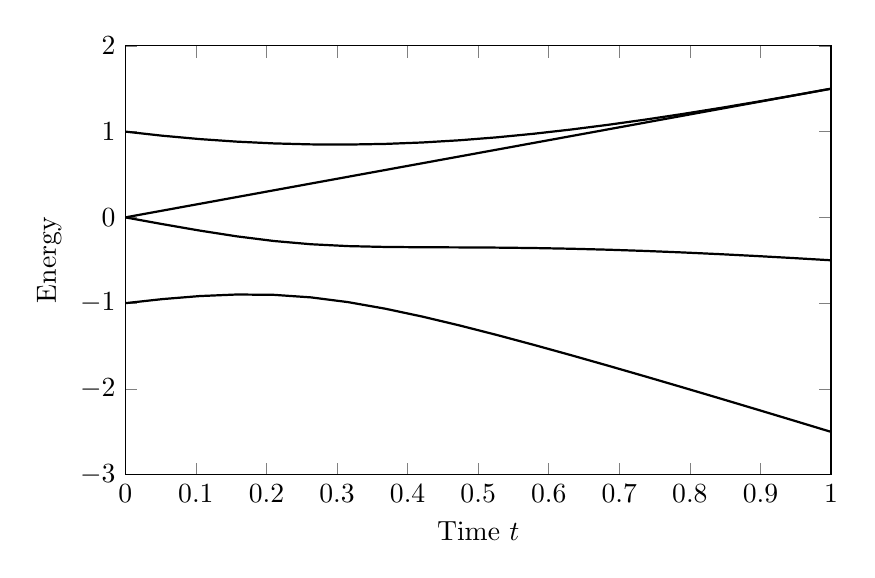
\begin{tikzpicture}
        \begin{axis}[width=300pt, height=200pt, xmin=0.0, xmax=1.0, ymin=-3.0, ymax=2.0, xlabel={Time $t$}, ylabel={Energy}]
        \addplot[color=black, style=thick] coordinates { (0.0, -0.9999999999999999) (0.05263157894736842, -0.9523709687365246) (0.10526315789473684, -0.9171551656149908) (0.15789473684210525, -0.8988902776352161) (0.21052631578947367, -0.902774337330783) (0.2631578947368421, -0.9325565467723903) (0.3157894736842105, -0.9879096804231118) (0.3684210526315789, -1.0644830596746586) (0.42105263157894735, -1.1566536920481425) (0.47368421052631576, -1.2596972717477464) (0.5263157894736842, -1.370291311607859) (0.5789473684210527, -1.4862367375212715) (0.631578947368421, -1.6060848989659724) (0.6842105263157894, -1.728862983979883) (0.7368421052631579, -1.8538994638777901) (0.7894736842105263, -1.9807172102402149) (0.8421052631578947, -2.1089678635823055) (0.894736842105263, -2.2383907612655682) (0.9473684210526315, -2.36878658494642) (1.0, -2.5) };
        \addplot[color=black, style=thick] coordinates { (0.0, -3.133653082431032e-16) (0.05263157894736842, -0.07846157972332896) (0.10526315789473684, -0.15359072699892687) (0.15789473684210525, -0.22091294387268887) (0.21052631578947367, -0.27530977951769803) (0.2631578947368421, -0.3131303200581205) (0.3157894736842105, -0.3347845586376573) (0.3684210526315789, -0.34463104721610927) (0.42105263157894735, -0.34816187488442163) (0.47368421052631576, -0.34978678017612674) (0.5263157894736842, -0.3523210442002797) (0.5789473684210527, -0.35729346785029376) (0.631578947368421, -0.3653756854207789) (0.6842105263157894, -0.37672120820949506) (0.7368421052631579, -0.39119647600518315) (0.7894736842105263, -0.4085278091571906) (0.8421052631578947, -0.42838960151895766) (0.894736842105263, -0.45045372964814256) (0.9473684210526315, -0.4744146411830131) (1.0, -0.5) };
        \addplot[color=black, style=thick] coordinates { (0.0, 2.1064402541011205e-17) (0.05263157894736842, 0.07894736842105263) (0.10526315789473684, 0.15789473684210525) (0.15789473684210525, 0.23684210526315785) (0.21052631578947367, 0.31578947368421045) (0.2631578947368421, 0.39473684210526316) (0.3157894736842105, 0.47368421052631593) (0.3684210526315789, 0.5526315789473684) (0.42105263157894735, 0.6315789473684211) (0.47368421052631576, 0.7105263157894737) (0.5263157894736842, 0.789473684210526) (0.5789473684210527, 0.868421052631579) (0.631578947368421, 0.9473684210526314) (0.6842105263157894, 1.0263157894736838) (0.7368421052631579, 1.1052631578947363) (0.7894736842105263, 1.1842105263157896) (0.8421052631578947, 1.2631578947368425) (0.894736842105263, 1.342105263157895) (0.9473684210526315, 1.4210526315789476) (1.0, 1.5) };
        \addplot[color=black, style=thick] coordinates { (0.0, 1.0000000000000002) (0.05263157894736842, 0.9518851800388011) (0.10526315789473684, 0.9128511557718124) (0.15789473684210525, 0.882961116244747) (0.21052631578947367, 0.8622946431642704) (0.2631578947368421, 0.8509500247252475) (0.3157894736842105, 0.8490100285344528) (0.3684210526315789, 0.8564825279433994) (0.42105263157894735, 0.8732366195641426) (0.47368421052631576, 0.8989577361343996) (0.5263157894736842, 0.933138671597613) (0.5789473684210527, 0.975109152739986) (0.631578947368421, 1.024092163334119) (0.6842105263157894, 1.0792684027156936) (0.7368421052631579, 1.139832781988236) (0.7894736842105263, 1.2050344930816148) (0.8421052631578947, 1.2741995703644204) (0.894736842105263, 1.3467392277558163) (0.9473684210526315, 1.4221485945504868) (1.0, 1.5) };
        \end{axis}
    \end{tikzpicture} \]
    During the annealing process, the state of the quantum system follows the lower line with high probability, resulting in the optimal solution $x_1 = x_2 = 1$ to the optimization problem.
\end{example}

\begin{topic}{abelian-hidden-subgroup-algorithm}{abelian hidden subgroup algorithm}
    The \textit{hidden subgroup problem} is the following problem.

    \textbf{Problem}: Given a group $G$ and a function $f \colon G \to S$ for some finite set $S$ such that there exists some subgroup $H \subseteq G$ for which $f(x) = f(y)$ if and only if $x H = y H$. Determine $H$.

    The \emph{abelian hidden subgroup algorithm} is a quantum algorithm to solve the hidden subgroup problem when $G$ is finite and abelian.

    \textbf{Algorithm}:
    Any finite group $G$ is of the form $(\ZZ / N_1 \ZZ) \times \cdots \times (\ZZ / N_k \ZZ)$ for some integers $N_j > 1$.
    Note that any character of $G$ is of the form
    \[ \chi_g (x) = \exp \left( \textstyle\sum_{j = 1}^{k} \frac{2 \pi i}{N_j} x_j g_j \right) \]
    for some $g = (g_1, \ldots, g_k) \in G$.
    Hence, the tensor product of \tref{quantum-fourier-transform}{quantum Fourier transforms}
    \[ F_{N_1} \otimes \cdots \otimes F_{N_k} \quad \textup{ precisely maps } \quad \ket{g} \mapsto \frac{1}{\sqrt{|G|}} \sum_{x \in G} \chi_g(x) \ket{x} . \]
    \begin{enumerate}[label=(\arabic*)]
        \item Start with the state $\ket{0} \ket{0}$, where the two registers have dimension $|G|$ and $|S|$, respectively. In particular, the basis states of the first register are $\ket{g}$ for $g \in G$, and those of the second register are $\ket{s}$ for $s \in S$.
        \item Create a uniform superposition over $G$ in the first register, to obtain the state $\frac{1}{\sqrt{|G|}} \sum_{g \in G} \ket{g} \ket{0}$.
        \item Compute $f$ in superposition to obtain the state $\frac{1}{\sqrt{|G|}} \sum_{g \in G} \ket{g} \ket{f(g)}$.
        \item Measure the second register to obtain some value $f(g)$ for some $g \in G$. The first register will collapse to a superposition over all $g' \in G$ such that $f(g') = f(g)$, that is, such that $g' \in g + H$. Hence, we are left with the state $\frac{1}{\sqrt{|H|}} \sum_{h \in H} \ket{g + h}$.
        \item Apply $F_{N_1} \otimes \cdots \otimes F_{N_k}$ to obtain the state
        \[ \begin{aligned}
            \frac{1}{\sqrt{|H| |G|}} \sum_{h \in H} \sum_{x \in G} \chi_{g + h}(x) \ket{x}
                = \frac{1}{\sqrt{|H| |G|}} \sum_{x \in G} \chi_g(x) \sum_{h \in H} \chi_h(x) \ket{x}
                = \sqrt{\frac{|H|}{|G|}} \sum_{\substack{x \in H^\perp}} \chi_g(x) \ket{x} ,
        \end{aligned} \]
        where $H^\perp = \{ x \in G \mid \chi_x(h) = 1 \textup{ for all } h \in H \}$, and where the last equality can be shown using the \href{/math-definitions/#RT:first-orthogonality-theorem}{first orthogonality theorem}.
        \item Measure the state. This yields some uniformly distributed element $x \in H^\perp$. Each such element corresponds to a constraint on $H$, because $\chi_x(h) = 1$ for all $h \in H$. Generating a small number of such elements will give sufficient information to find the generators of $H$.
    \end{enumerate}
\end{topic}

\begin{example}{abelian-hidden-subgroup-algorithm}
    The hidden subgroup problem reduces to \tref{simon-algorithm}{Simon's problem} for $G = (\ZZ / 2\ZZ)^{n}$ and $H = \{ 0, s \}$ for some $s \in G$. In fact, the abelian hidden subgroup algorithm reduces precisely to Simon's algorithm.
\end{example}
